\documentclass{article}

% Language setting
% Replace `english' with e.g. `spanish' to change the document language
\usepackage[english]{babel}

% Set page size and margins
% Replace `letterpaper' with`a4paper' for UK/EU standard size
\usepackage[a4paper,top=2cm,bottom=2cm,left=3cm,right=3cm,marginparwidth=1.75cm]{geometry}

% Useful packages
\usepackage{float}
\usepackage{amsmath}
\usepackage{graphicx}
\usepackage[colorlinks=true, allcolors=blue]{hyperref}

\title{\LARGE GRM: Coursework Assignment}
\author{Luis Angel Montoya Franco}

\begin{document}
\maketitle

\begin{abstract}
This article is about the relationship between the recovery time of patients elapsed between the time at a drug was discontinued and the time at the systolic blood pressure returns to 100 mm Hg.
\end{abstract}

\section{Introduction}

The data used for this analysis was taken from a clinical trial to study a hypotensive drug used to lower the blood pressure during operations. The question of interest is the extent to which the recovery time depends on the quantity of drug used and the level to which blood pressure was lowered during hypotension. 

The data consist in fifty three observations, each observation has three elements, which are:
\begin{itemize}
    \item \(x_1\) = log(quantity of drug used, in mg)
    \item \(x_2\) =  mean level of systolic blood pressure during hypotension, in mm Hg
    \item y = recovery time in minutes
\end{itemize}
Throughout  this analysis, the statistical software R was used to do the calculations and plots. 
\section{Exploratory analysis}

First of all, the three variables are analysed independently by plotting the histograms for each one of them, the histograms are shown below


\begin{figure}[H]
\centering
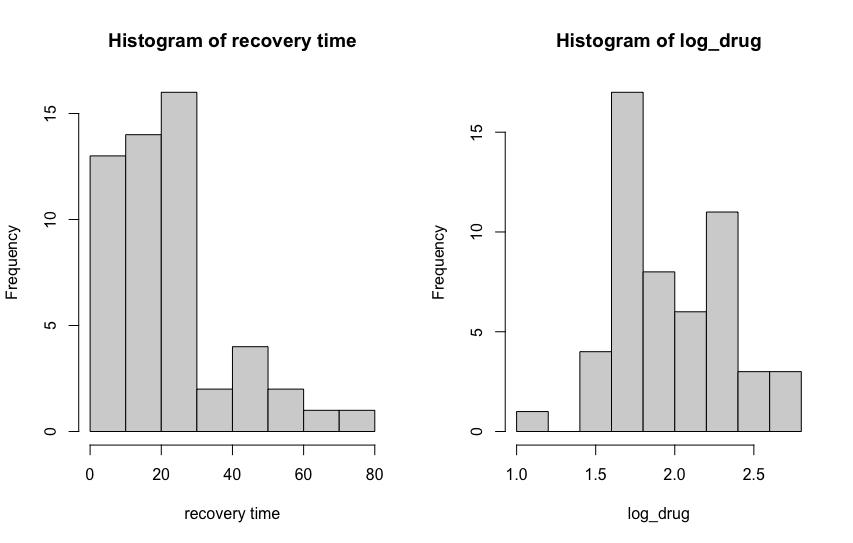
\includegraphics[width=0.8\textwidth]{hx1x2.png}
\caption{\label{fig:frog} Histogram of $x_2$ on the left and $x_1$ on the right}
\end{figure}


\begin{figure}[H]
\centering
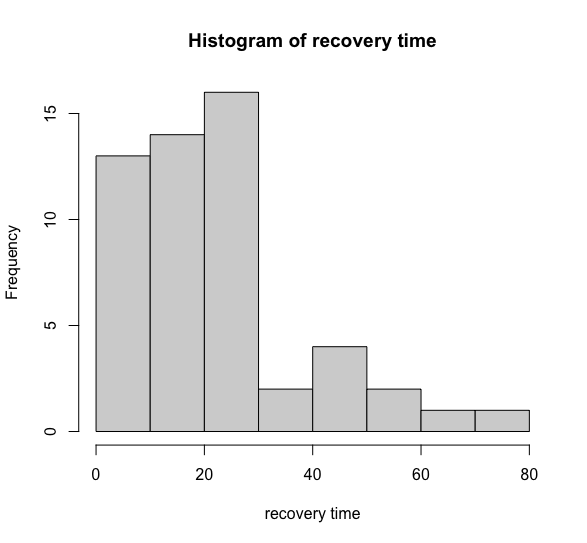
\includegraphics[width=0.6\textwidth]{hrt.png}
\caption{\label{fig:frog} Histogram of recovery time}
\end{figure}

In addition, two-dimensional plots of the response variable against the independent variables were made in order to see any linear relationship between them. These charts are presented below

\begin{figure}[H]
\centering
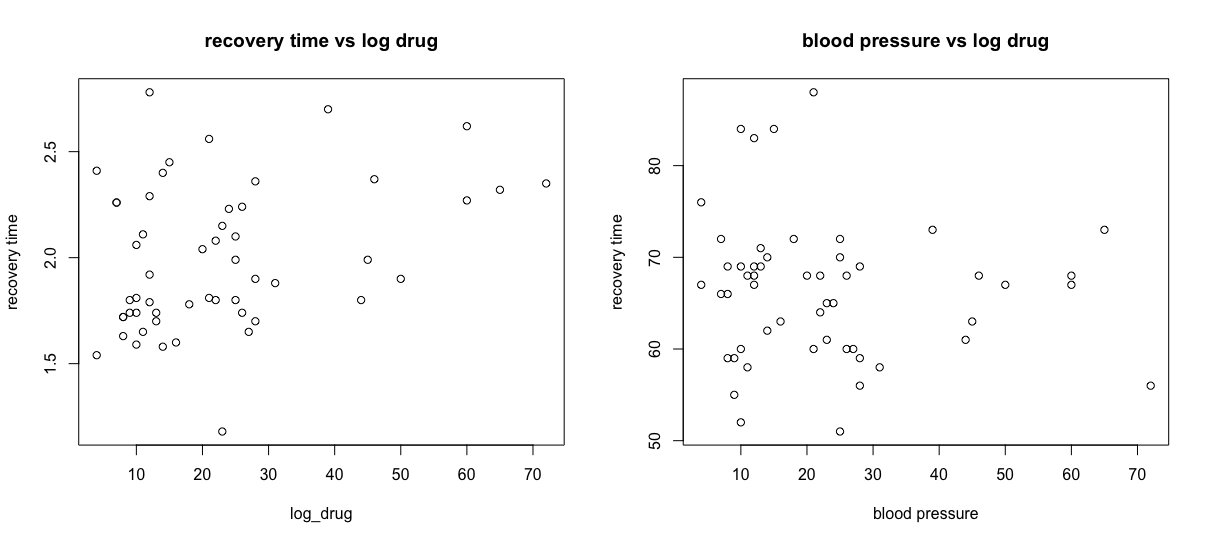
\includegraphics[width=1\textwidth]{evsr.png}
\caption{\label{fig:frog} Scatter plots of the response variable against the independent variables}
\end{figure}

In order to see a better linear relationship between the response variable and the independent variables, some transformations to stabilize the variance were applied, such transformations were the natural logarithm of y variable, and apply the exponential function to \(x_1\) variable. Once these transformations have been applied, it is possible to plot the two-dimensional charts again. These charts are shown below

\begin{figure}[H]
\centering
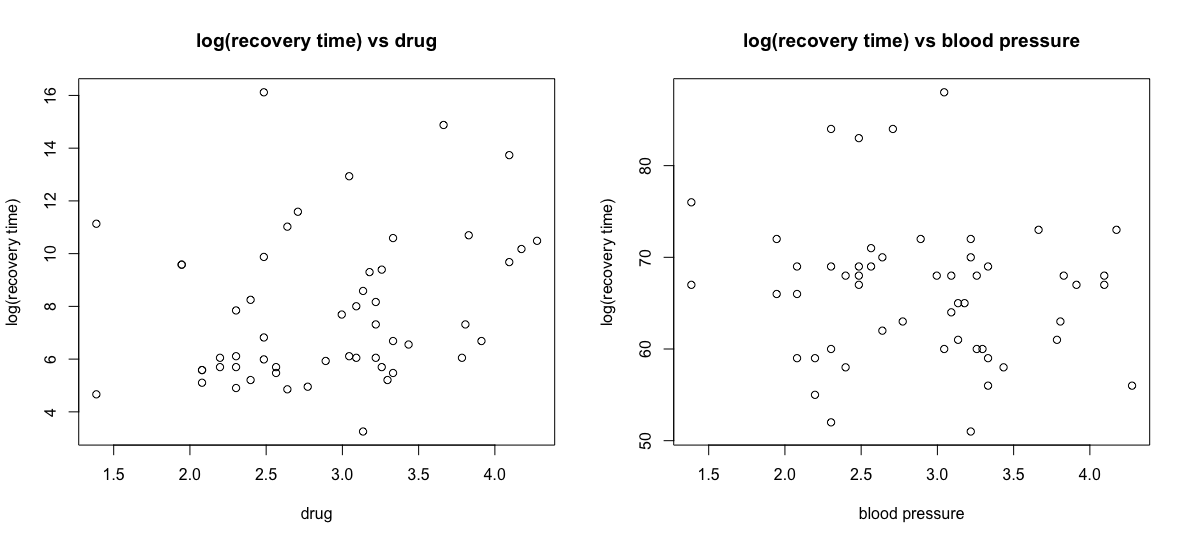
\includegraphics[width=1\textwidth]{tvs.png}
\caption{\label{fig:frog} Scatter plots of the response variable against the independent variables after applying transformations}
\end{figure}



\section{Linear modeling}

Assuming that the recovery time can be calculated as a linear combination of the variables $x_1$ and $x_2$, a linear model can be fitted, in other words, it is possible to express the the observations in the following way

$$\begin{bmatrix} y^{(1)} \\y^{(2)} \\... \\ y^{(n)}  \end{bmatrix} = 
\begin{bmatrix} 1 & x_1^{(1)} &  x_2^{(1)}\\1 &  x_1^{(2)}  & x_2 ^{(2)}\\... & ... & ... \\ 
1 &  x_1^{(n)}  & x_2 ^{(n)} \end{bmatrix} \begin{bmatrix} \beta_0 \\\beta_1 \\ \beta_2 \end{bmatrix} +\begin{bmatrix} \epsilon^{(1)} \\ \epsilon^{(2)} \\ ... \\ \epsilon^{(n)} \end{bmatrix}
$$ \
where
\begin{itemize}
    \item $y^{(i)}$ is the i-th observation of the variable y
     \item $x_1^{(i)}$ is the i-th observation of the variable $x_1$
     \item $x_2^{(i)}$ is the i-th observation of the variable $x_2$
     \item $\beta_0$ is the intercept
     \item $\beta_1$ is the coefficient of the variable $x_1$
     \item $\beta_2$ is the coefficient of the variable $x_2$
     \item $\epsilon^{(i)}$ is the error of the the model for the i-th observation
\end{itemize}
The parameters of this model are \(\beta_0\), \(\beta_1\) and \(\beta_2\) which can be estimated using least squares. \\

As mentioned in the previous sections, some transformations were applied to the data, in order to fulfill the normality criteria in the residuals, such transformations were:

\begin{itemize}
    \item log(recovery time)
    \item exp(logarithm of the drug)
\end{itemize}

thus, each observation is modeled in the following way 
$$log(y^{(i)}) = \beta_0 + \beta_1exp(x_1^{(i)})+ \beta_2x_2^{(i)} + \epsilon^{(i)}   $$


\section{Summary of the model}

Once the model is fitted, R provides a summary of it. This summary shows some key aspects of the model, such as the Descriptive statistics of the residuals, the estimated parameters of the model, their standard error, the value of the statistic and p-value for a t-test , where the null hypothesis is that each parameter is equal to 0. If the p-value is less than a significance level $\alpha$ (which is 0.05), it can be said that the null hypothesis can be rejected, in other words, it can be said that there is enough statistical evidence to say, that it exists a relationship between the corresponding variable of the coefficient that is being tested with the response variable. \\
The summary of the model described in the previous section is presented below.
 

\begin{figure}[H]
\centering
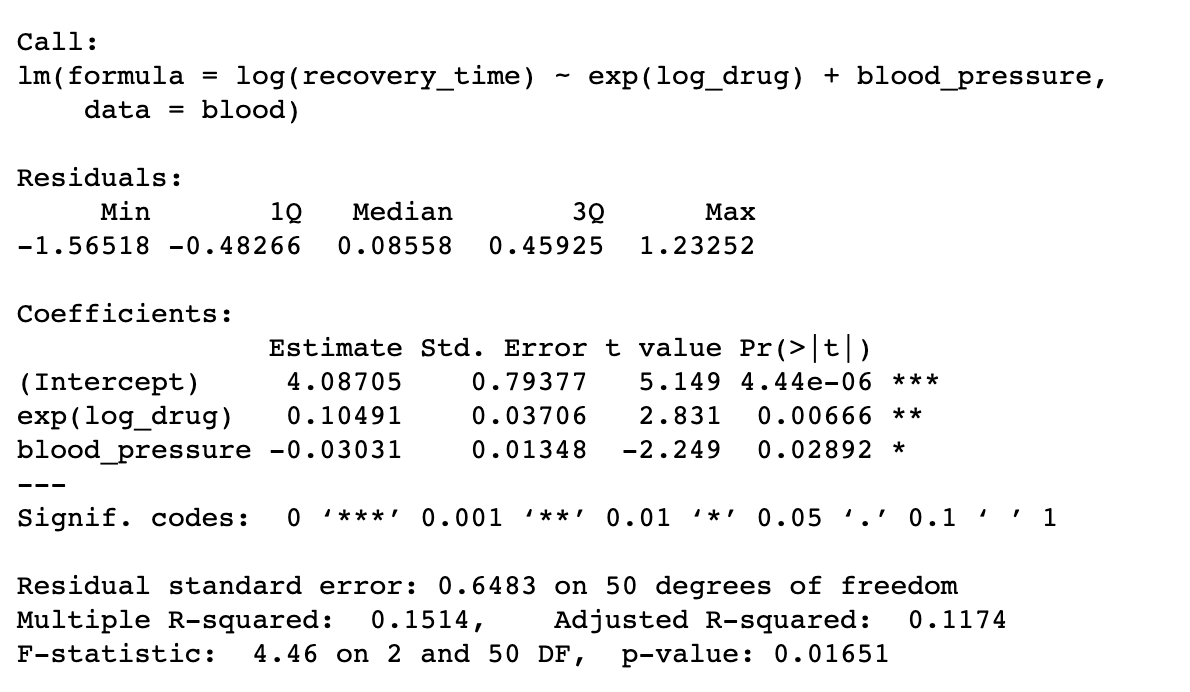
\includegraphics[width=0.8\textwidth]{sm.png}
\caption{\label{fig:frog} Summary of the model $log(y^{(i)}) = \beta_0 + \beta_1exp(x_1^{(i)})+ \beta_2x_2^{(i)} + \epsilon^{(i)}   $}
\end{figure}

Thus, according to the summary, all of the p-values for the coefficients are less than significance level, therefore, it can be said that there exists a linear relationship between the recovery time, the amount of drug used and the blood pressure. 

\section{Assumptions of the model}

The linear model applied previously has different assumptions that must be fulfilled, in case they are not fulfilled, another model type of model should be used.  

The main assumptions of the linear model used, are 

\begin{itemize}
    \item The errors follow a normal distribution with zero mean
    \item Constant variance
\end{itemize}
R also provides more plots about the model that can help to prove this assumptions. 

The first chart to take a look at, is the "residuals vs fitted" plot, where it can be seen it the residuals have approximately zero expectation. The plot can be seen below

\begin{figure}[H]
\centering
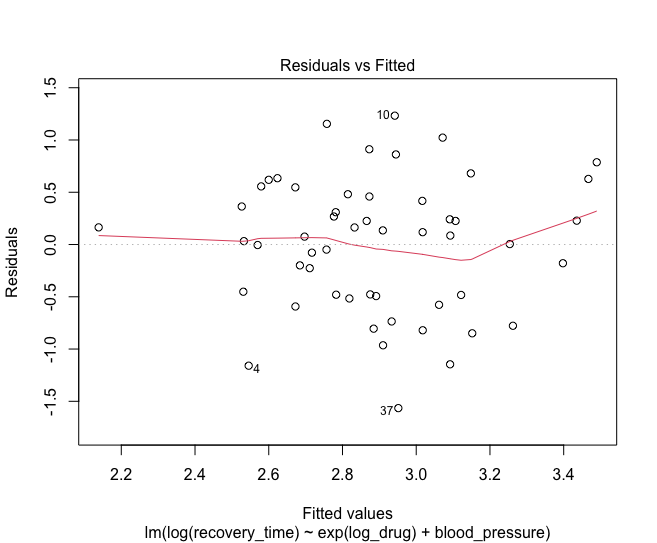
\includegraphics[width=0.5\textwidth]{rvsf.png}
\caption{\label{fig:frogg} Residuals vs fitted }
\end{figure}

The next plot provided by R is the "normal Q-Q"plot which shows whether the residuals follow a normal distribution or not, if they do, the point will form a line. The chart is presented below

\begin{figure}[H]
\centering
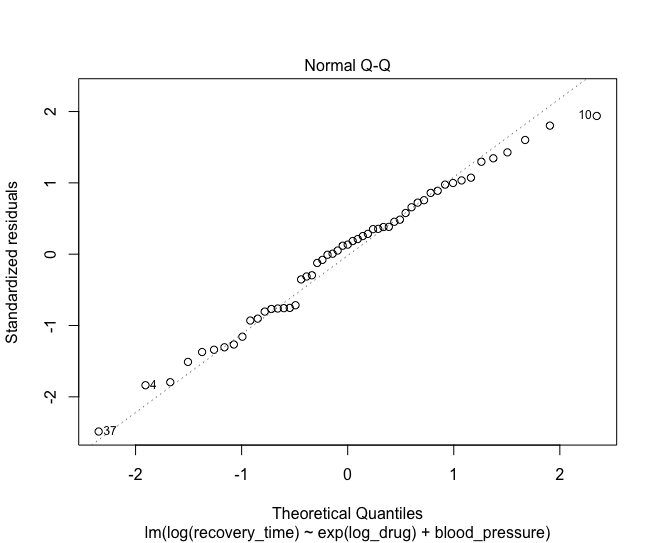
\includegraphics[width=0.5\textwidth]{qq.png}
\caption{\label{fig:frogg} Normal Q-Q plot }
\end{figure}


In addition, a histogram of the residuals is presented below

\begin{figure}[H]
\centering
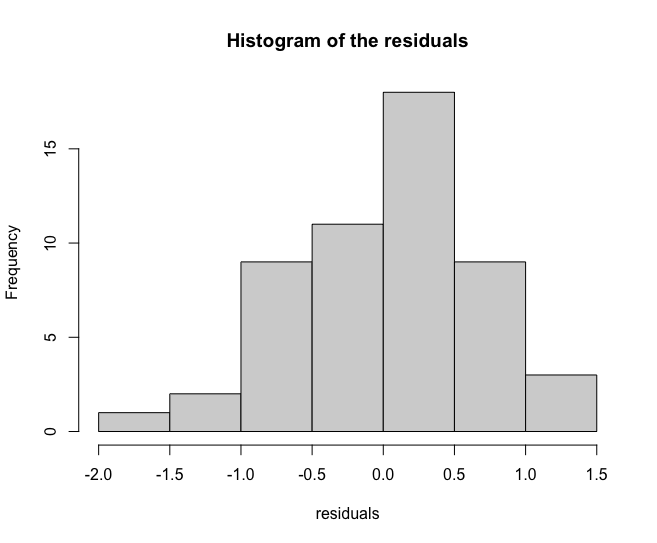
\includegraphics[width=0.5\textwidth]{hr.png}
\caption{\label{fig:frogg} Histogram of the residuals }
\end{figure}

Finally, a Shapiro-Wilk test was made, this test contrasts whether a set of observations comes from a normal distribution or not where the null hypothesis is that the observations come from a normal distribution. The p-value obtained by the test is 0.693, therefore, the null hypothesis can not be rejected. \\
\\
The last chart to analyse is the "scale-location" plot, which allows to see whether the variance is constant or not. The chart is presented below

\begin{figure}[H]
\centering
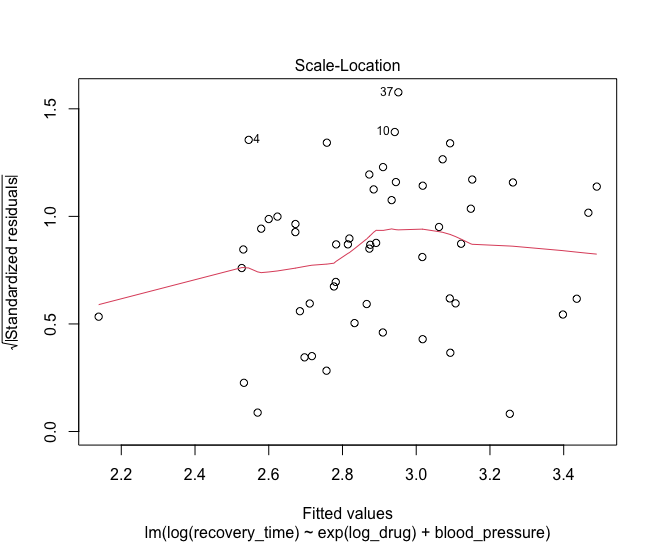
\includegraphics[width=0.6\textwidth]{sl.png}
\caption{\label{fig:frogg} Scale-Location}
\end{figure}
In this chart, the red line must be approximately horizontal to ensure that the variance is constant, in other words, that the homoskedasticity criteria is fulfilled. In the chart, although the red line is not a perfect straight line, it is not a polynomial or exponential curve, thus, it can be said that the variance of the residuals is constant. 

\section{Confidence interval}
Finally, it is of interest to get a 95\% confidence interval for the recovery time when the  log of the quantity of drug is 2.00 and the mean level of systolic blood pressure during hypotension is 75mm Hg.
\\
Using the model for these levels of drug and blood pressure, it is possible to get a point estimation of the recovery time and a confidence interval, these estimations are

\begin{itemize}
    \item Point estimation: 13.31501
    \item Confidence interval (9.790195, 18.1089)
\end{itemize}

\newpage
\section{Appendix}

Here is the code used to get the results described in this document. 

\begin{verbatim}setwd("/Users/angel/OneDrive - University of Edinburgh/Semestre 1/GRM/GRM_assigment1/")
blood <- read.table('datasets/Bloodpressure.txt',head=T)

par(mfrow=c(1,2))
hist(blood$recovery_time,  xlab = "recovery time", main = "Histogram of recovery time")
hist(blood$log_drug, xlab = "log_drug", main = "Histogram of log_drug")
hist(blood$blood_pressure, xlab = "blood pressure", main = "Histogram of blood pressure")

par(mfrow=c(1,2))
plot(blood$recovery_time, blood$log_drug, xlab="log_drug", ylab = "recovery time")
title("recovery time vs log drug")
plot(blood$recovery_time, blood$blood_pressure,  xlab="blood pressure", ylab = "recovery time")
title("blood pressure vs log drug")


par(mfrow=c(1,2))
plot(log(blood$recovery_time),exp(blood$log_drug),xlab="drug", ylab = "log(recovery time)")
title("log(recovery time) vs drug")
plot(log(blood$recovery_time), blood$blood_pressure,  xlab="blood pressure", ylab = "log(recovery time)")
title("log(recovery time) vs blood pressure")


#Simple linear regession model 
Model1 <- lm(formula = log(recovery_time) ~ exp(log_drug) + blood_pressure, data =blood)
summary(Model1)


par(mfrow = c(2, 2))
plot(Model1)

plot(Model1)

par(mfrow = c(1, 1))
hist(Model1$res,xlab="residuals",  main = "Histogram of the residuals", )


new.data = data.frame(log_drug=2, blood_pressure=75 )

interval <- predict(Model1, newdata = new.data, interval = "confidence", level = 0.95)
interval

exp(interval)
\end{verbatim}















\end{document}
